% Native, editable teaching diagrams. R01--R18; no appendix material.
\newcommand{\RestMap}[1]{%
  \node[circle,draw=teal,fill=pale,minimum size=7mm,font=\small] (r0) at (0,1) {0};
  \node[circle,draw=teal,fill=pale,minimum size=7mm,font=\small] (r1) at (1.7,2.2) {1};
  \node[circle,draw=amber,fill=amber!12,minimum size=7mm,font=\small] (r2) at (3.7,2.2) {2};
  \node[circle,draw=teal,fill=pale,minimum size=7mm,font=\small] (r3) at (5.5,1) {3};
  \node[circle,draw=teal,fill=pale,minimum size=7mm,font=\small] (r4) at (3.7,-.2) {4};
  \node[circle,draw=amber,fill=amber!12,minimum size=7mm,font=\small] (r5) at (1.7,-.2) {5};
  \draw[slate] (r0)--(r1);
  \draw[red,dashed,very thick] (r1)--node[midway,fill=white,text=red,font=\large] {$\times$}(r2);
  \draw[slate] (r2)--(r3)--(r4);
  \draw[slate] (r2)--(r5);
  \draw[amber,dashed,thick] (r1)--node[left,font=\scriptsize,fill=white]{100 kW}(r5);
  \draw[amber,dashed,thick] (r0) to[out=-75,in=205] (r4);
  \node[font=\scriptsize,text=amber,align=center] at (0,-.55) {tie 0--4\\#1 kW};
  \node[font=\scriptsize,above=1mm of r1] {40 kW};
  \node[font=\scriptsize,above=1mm of r2,text=amber] {60 kW, critical};
  \node[font=\scriptsize,right=1mm of r3] {70 kW};
  \node[font=\scriptsize,below=1mm of r4] {50 kW};
  \node[font=\scriptsize,below=1mm of r5,text=amber] {30 kW, critical};
  \node[font=\scriptsize,left=1mm of r0] {source};
}

\begin{frame}[t]{A fault changes the paths that are available}
\label{f:R01}
\begin{columns}[T,onlytextwidth]
\column{.59\textwidth}
\begin{tikzpicture}[scale=.93,transform shape]
\RestMap{40}
\uncover<2->{\node[box,text width=5.5cm] at (2.6,-1.55) {Fault 1--2 stays isolated.\\Check ties only after isolation.};}
\end{tikzpicture}
\column{.39\textwidth}
\Idea{A small, transparent fixture}{Six nodes; five loads; one failed segment; two optional ties. Amber nodes have higher service priority.}
\Question{Can we simply reconnect the failed segment?}
\Answer{No. Its availability is fixed to zero. Planning must find another admissible path.}
\end{columns}
\Source{Fresh classroom fixture: Classroom\_Labs L6; src/standard\_formulations.py. Restoration context: \href{https://doi.org/10.1109/TPWRS.2017.2720122}{Chen et al., IEEE TPWRS, 2018}.}
\Bridge{What can each alternative path carry?}
\note{Begin with the physical picture, not an optimization acronym. Node zero is the available source. The interrupted segment connects nodes one and two, and is unavailable throughout the experiment. The dashed amber links are candidate ties, not commands already issued. Nodes two and five are designated critical in this classroom fixture. Explain that the drawing is a six-node active-power transport example, not a reduced drawing of the full Greensboro feeder. Its purpose is to expose the decisions clearly enough to check them by hand. Ask the audience to point to the failed segment and identify a route that avoids it. Reveal the isolation statement before discussing any restoration action. A real switching procedure additionally needs protection, equipment status, work permits and operator authority, which this static fixture does not establish.}
\end{frame}

\begin{frame}[t]{Two ties create choices, with different bottlenecks}
\label{f:R02}
\begin{columns}[T,onlytextwidth]
\column{.60\textwidth}
\begin{tikzpicture}[scale=.93,transform shape]
\RestMap{40}
\uncover<2->{\draw[teal,line width=2pt,->] (r0)--(r1);\draw[teal,line width=2pt,->] (r1)--(r5);\draw[teal,line width=2pt,->] (r5)--(r2);}
\uncover<3->{\draw[blue,line width=2pt,->] (r0) to[out=-75,in=205] (r4);}
\end{tikzpicture}
\column{.38\textwidth}
\Idea{Follow the power}{The route $0\!\to\!1\!\to\!5\!\to\!2$ uses the 100 kW tie. The other tie has only 40 kW in this first case.}
\Question{Can the 40 kW tie pick up the entire 50 kW load at node 4?}
\uncover<3->{\textcolor{red}{No: $50>40$.} Loads are indivisible here; partial pickup is excluded.}
\end{columns}
\Source{Fixture and binary pickup assumption: Classroom\_Labs L6; standard\_formulations.restoration\_graph. Blue and teal paths are explanatory alternatives, not a switching sequence.}
\Bridge{Does an energized node have to serve its local load?}
\note{Trace the teal route with a pointer while it appears. The hundred-kilowatt tie between nodes one and five must carry the downstream demand that the chosen tree places behind it. Node one's own forty-kilowatt demand can be supplied before that bottleneck. The other tie supplies the lower side of the diagram, but at forty kilowatts it cannot pick up the fifty-kilowatt block at node four. That conclusion relies on the all-or-nothing pickup assumption. It would change if loads could be divided into smaller controllable groups. The colors describe routes for reasoning; the slide does not certify a safe temporal switching sequence. Ask participants to distinguish a branch rating from the total rating of the source. The next distinction is between energizing a bus so power can pass through it and reconnecting that bus's local demand.}
\end{frame}

\begin{frame}[t]{A node can carry power while its load stays disconnected}
\label{f:R03}
\begin{columns}[T,onlytextwidth]
\column{.60\textwidth}
\begin{tikzpicture}[scale=.93,transform shape]
\RestMap{40}
\draw[teal,line width=1.7pt] (r0)--(r1)--(r5)--(r2)--(r3);
\node[box,text width=5.7cm] at (2.7,-1.55) {Example: serve nodes 1, 3, 5; pass through node 2.};
\uncover<2->{\node[draw=red,fill=white,rounded corners,font=\scriptsize,align=center] at (4.5,3.35) {node 2 energized\\local 60 kW disconnected};}
\end{tikzpicture}
\column{.38\textwidth}
\Idea{Two different binary decisions}{$y_i=1$: node $i$ is energized.\par $s_i=1$: its load is picked up.\par\smallskip We require $s_i\le y_i$.}
\Question{Why is equality $s_i=y_i$ too restrictive?}
\Answer{It would forbid a useful transit node whose own load remains shed.}
\end{columns}
\Source{Original schematic of a feasible six-node plan; binary pickup/energization model in src/standard\_formulations.py.}
\Bridge{How do we compare feasible pickup decisions?}
\note{This is an important modeling distinction that is easy to miss when a diagram uses one color for everything. The illustrated path can carry power through node two while leaving its sixty-kilowatt demand disconnected. In the example, the tie between one and five carries thirty kilowatts for node five plus seventy for node three, exactly one hundred kilowatts. Node one's forty kilowatts are supplied upstream. The total picked up is therefore one hundred forty kilowatts. Define the energized variable and the pickup variable in words before showing their inequality. The figure is an explicit feasible explanation of the unweighted service level, not a claim that every optimizer returns this exact edge list. Different optimal trees can exist. Invite participants to explain why a transit node still needs valid energized connectivity even when its local pickup variable is zero.}
\end{frame}

\begin{frame}[t]{A capacity budget turns priorities into a real choice}
\label{f:R04}
\begin{columns}[T,onlytextwidth]
\column{.54\textwidth}
\begin{tikzpicture}[x=.047cm,y=1cm]
\draw[slate] (0,0) rectangle (100,.65);
\fill[amber!70] (0,0) rectangle (60,.65);
\fill[teal!60] (60,0) rectangle (90,.65);
\node[font=\small] at (30,.32) {node 2: 60};
\node[font=\scriptsize] at (75,.32) {5: 30};
\node[font=\small,above] at (50,.8) {Critical pair: $60+30=90$ kW};
\uncover<2->{\fill[slate!25] (0,-1.45) rectangle (70,-.8);\fill[teal!60] (70,-1.45) rectangle (100,-.8);\draw[slate] (0,-1.45) rectangle (100,-.8);\node[font=\small] at (35,-1.12) {node 3: 70};\node[font=\scriptsize] at (85,-1.12) {5: 30};\node[font=\small,below] at (50,-1.6) {Largest total: $70+30=100$ kW};}
\end{tikzpicture}
\column{.43\textwidth}
\Idea{The 100 kW tie is the budget}{Both choices also serve node 1's 40 kW upstream.\par Critical pair: total 130; critical 90.\par Largest total: total 140; critical 30.}
\Question{Which outcome should a critical-service policy prefer?}
\Answer{The answer depends on the stated objective, not on how persuasive its explanation sounds.}
\end{columns}
\Source{Hand-checkable choices at tie 0--4 capacity 40 kW; exact optima confirmed by Classroom\_Labs L6. Bars represent kW, not physical line lengths.}
\Bridge{How do we put that service policy into mathematics?}
\note{Use the bars as a budget, with each indivisible load consuming part of the hundred-kilowatt tie capacity. The top choice carries the two critical loads, sixty plus thirty kilowatts, leaving ten unused. That unused capacity cannot serve any remaining complete load block. The bottom choice uses all one hundred kilowatts to carry seventy plus thirty. Both plans also serve forty kilowatts at node one upstream, so their total service is one hundred thirty and one hundred forty respectively. Ask for a preference before revealing the policy interpretation. The lower total service is not evidence that the weighted optimizer failed. It can be the intended consequence of protecting critical demand. Equally, the higher total service is not a mistake under an explicitly unweighted objective. This prepares a fair comparison: same feasible network, transparent objectives, and both total and critical service reported.}
\end{frame}

\begin{frame}[t]{Compare outcomes before comparing algorithms}
\label{f:R05}
\begin{center}
\begin{tabular}{lrrr}
\toprule
Same 40 kW tie case & Total served & Critical served & Critical share served\\
\midrule
Maximize total kW & 140 kW & 30 kW & $30/90$\\
\uncover<2->{Maximize weighted kW & 130 kW & 90 kW & $90/90$}\\
\bottomrule
\end{tabular}
\end{center}
\Idea{What the experiment establishes}{Changing the service objective changes who benefits. It does not establish an advantage caused by an LLM or by the word ``agentic.''}
\Question{What must stay matched to isolate an agentic workflow effect?}
\Answer{The objective, candidate tools, physical limits, information and verification rules.}
\Source{Fresh six-node experiment: Classroom\_Labs L6, weighted MILP versus unweighted exact enumeration; both use the same feasible constraints.}
\Bridge{What does a priority weight of ten actually mean?}
\note{Keep the table visible long enough for participants to read both columns. Reporting only total service would conceal the reason the weighted formulation was chosen. Reporting only critical service would conceal the sacrifice in ordinary service. The first comparison intentionally changes the objective, so it is a policy comparison. It is not a controlled test of language-model orchestration. The unweighted baseline is solved exactly by enumeration on the same small network and constraints; it is not a deliberately weak random baseline. The weighted MILP is also checked against exhaustive enumeration. Later we will compare a fixed supervisor and an LLM supervisor with matched objectives and tools, using a separate archived feeder experiment. Ask the audience to list what must be held equal in that later comparison. This distinction helps them avoid attributing every favorable result to the framework.}
\end{frame}

\begin{frame}[t]{The objective is an explicit, inspectable service policy}
\label{f:R06}
\[
\max \sum_{i=1}^{5} w_i d_i s_i,
\qquad w_2=w_5=10,\qquad w_1=w_3=w_4=1.
\]
\begin{columns}[T,onlytextwidth]
\column{.48\textwidth}
\Idea{Critical-pair choice}{$10(60+30)+40=\mathbf{940}$\par weighted kW; 130 actual kW.}
\column{.48\textwidth}
\uncover<2->{\Idea{Maximum-total choice}{$10(30)+70+40=\mathbf{410}$\par weighted kW; 140 actual kW.}}
\end{columns}
\small $d_i$: load demand in kW; $w_i$: dimensionless priority; $s_i\in\{0,1\}$: pickup.
\Question{Does weight ten guarantee critical-first service on every possible network?}
\Answer{No. Strict priority requires a lexicographic objective or a proven sufficiently large weight.}
\Source{Classroom priority policy: standard\_formulations.restoration\_graph. Weighted restoration objectives: \href{https://doi.org/10.1109/TPWRS.2017.2720122}{Chen et al., 2018}.}
\Bridge{Which constraints make a high-scoring plan physically admissible?}
\note{Read the expression aloud as demand multiplied by a priority and a pickup decision, then summed over loads. Distinguish actual kilowatts from the weighted score. The critical-pair plan earns nine hundred forty weighted kilowatts, while the illustrated maximum-total plan earns four hundred ten. The factor ten is an instructional policy choice, not an empirical estimate of a hospital's value or an industry-wide standard. A finite weight can be outweighed by sufficiently much ordinary demand, so it does not automatically encode strict critical-first restoration. If strict priority is required, solve critical service first and preserve that optimum in a second objective, or justify a bound on the weight. The planner should expose this assumption to the operator rather than letting an LLM silently invent priorities. Now move from scoring plans to checking which plans are feasible.}
\end{frame}

\begin{frame}[t]{Planning: binary pickup and topology decisions}
\label{f:R07}
\begin{columns}[T,onlytextwidth]
\column{.48\textwidth}
\begin{tabular}{ll}
\toprule Symbol & Meaning\\\midrule
$s_i\in\{0,1\}$ & load $i$ picked up\\
$y_i\in\{0,1\}$ & node $i$ energized\\
$z_e\in\{0,1\}$ & edge $e$ closed\\
$P_e\in\mathbb R$ & signed active flow, kW\\
$\bar P_e$ & edge capacity, kW\\\bottomrule
\end{tabular}
\column{.48\textwidth}
\begin{align*}
s_i&\le y_i, & y_0&=1,\\
z_{ij}&\le y_i, &z_{ij}&\le y_j,\\
z_{1,2}&=0.&&
\end{align*}
\uncover<2->{\Idea{Interpret each line}{Picked-up loads need energized nodes; closed edges need energized endpoints; the fault stays isolated.}}
\end{columns}
\Question{Which of these rules prevents a disconnected energized island?}
\Answer{None yet. Connectivity must be imposed separately.}
\Source{Fresh MILP implementation: src/standard\_formulations.py. Radiality and connectivity: \href{https://arxiv.org/abs/1912.05185}{Wang et al., 2020}.}
\Bridge{How do flow balance and capacity restrict pickup?}
\note{Introduce one decision type at a time and connect it to the preceding diagrams. The pickup variable describes demand, the energized variable describes the usable network, and the edge variable describes the selected topology. Signed flow needs an arbitrary reference orientation; a negative value simply means power travels the other way. The source is fixed energized, and the failed segment is fixed open. The endpoint constraints prevent a selected line from attaching to a node labeled de-energized. These are necessary logical conditions, but they do not prove that every energized node is reachable from the source. Pause on that omission. An isolated cycle could satisfy many local conditions while being impossible to supply. The next two slides add active-power transport and source connectivity. This modular construction explains what each constraint contributes rather than presenting one intimidating formulation without interpretation.}
\end{frame}

\begin{frame}[t]{Power balance says where every picked-up kilowatt comes from}
\label{f:R08}
\[
\underbrace{\sum_{e} A_{ie}P_e}_{\text{net active power entering node }i}
=\underbrace{d_i s_i}_{\text{picked-up demand}},\quad i\ne0,
\qquad -\bar P_e z_e\le P_e\le\bar P_e z_e.
\]
\begin{center}
\begin{tikzpicture}[node distance=1.4cm]
\node[box] (in) {100 kW in};
\node[box,right=of in] (node) {node 5};
\node[box,right=of node] (out) {70 kW onward};
\node[box,below=.55cm of node] (load) {30 kW picked up};
\draw[arrow] (in)--(node);\draw[arrow] (node)--(out);\draw[arrow] (node)--(load);
\end{tikzpicture}
\end{center}
\small $A_{ie}=+1$ for an edge entering $i$, $-1$ leaving it, zero otherwise.
\uncover<2->{\Idea{Know the model boundary}{This is lossless active-power transport. Voltage, reactive power, AC losses and protection are not certified.}}
\Source{Classroom\_Labs L6; active-transport formulation in src/standard\_formulations.py. This six-node model is separate from the archived feeder power-flow checks.}
\Bridge{How can we prove every energized node has a source path?}
\note{Use the small flow diagram to show that balance is bookkeeping with a physical interpretation. One hundred kilowatts arrive at node five, thirty are consumed locally, and seventy continue downstream. With the stated incidence convention, incoming flows enter positively and outgoing flows negatively. At an open edge, the binary variable is zero, forcing its flow to zero. At a closed edge, the same inequalities bound the magnitude by the rating. The source balance is handled as the supply needed to satisfy non-source demand. State the model limitation clearly: a feasible active-transport solution is not an AC security certificate. It ignores voltage, reactive power, losses and protection behavior. That simplicity is deliberate for a hand-checkable lesson. The later archived feeder result uses additional power-flow evidence, but must not be confused with this exact MILP fixture.}
\end{frame}

\begin{frame}[t]{Edge counts alone do not prove a source-connected tree}
\label{f:R09}
\begin{columns}[T,onlytextwidth]
\column{.43\textwidth}
\begin{tikzpicture}[every node/.style={circle,draw=slate,minimum size=6mm,font=\small}]
\node[fill=pale] (a) at (0,1) {0};\node (b) at (1.2,1) {1};
\node (c) at (2.8,1.7) {2};\node (d) at (2.1,.1) {3};\node (e) at (3.5,.1) {4};
\draw (a)--(b);\draw[red,thick] (c)--(d)--(e)--(c);
\node[draw=none,rectangle,align=center,font=\small] at (1.75,-.7) {5 nodes; 4 edges\\but an unsupplied cycle};
\end{tikzpicture}
\column{.55\textwidth}
\uncover<2->{\begin{align*}
\sum_e A_{ie}f_e&=y_i &&(i\ne0),\\
-5z_e\le f_e&\le5z_e,\\
\sum_e z_e&=\sum_i y_i-1.
\end{align*}}
\small $f_e$: fictitious connectivity flow, not electrical kW. Every energized non-source node consumes one unit. Five is the maximum number of such nodes.
\end{columns}
\Idea{Two jobs, two conditions}{Commodity flow proves reachability. Reachability plus the edge count gives a tree on the energized nodes.}
\Source{Original counterexample; single-commodity connectivity and radiality: \href{https://arxiv.org/abs/1912.05185}{Wang et al., 2020}; classroom MILP.}
\Bridge{How do we check a small MILP without trusting its solver blindly?}
\note{The left-hand counterexample is a separate five-node sketch, not the six-node restoration fixture. It has the familiar tree edge count but is disconnected: the source supplies one short component while three other nodes form a cycle. This makes the missing condition visible. Reveal the fictitious flow equations and explain that these units are proof tokens. Every energized non-source node must receive one token through selected edges, so an island without the source cannot satisfy the summed balances. The source provides the required tokens. The bound of five is enough because the classroom network has five non-source nodes. Once all selected energized nodes are connected, exactly one fewer edge than nodes eliminates cycles. Emphasize that this proves a static graph property. It does not address the time ordering of switching, transient stability or protection coordination.}
\end{frame}

\begin{frame}[t]{Verification uses an independent, exhaustive small-case check}
\label{f:R10}
\begin{center}
\begin{tikzpicture}[node distance=.7cm]
\node[box,text width=3.1cm] (m) {HiGHS MILP\\weighted optimum};
\node[box,text width=3.7cm,right=of m] (e) {Enumerate pickup and edges\\check paths, trees and ratings};
\node[box,text width=3.1cm,right=of e] (v) {Compare objectives\\and feasibility};
\draw[arrow] (m)--(e);\draw[arrow] (e)--(v);
\end{tikzpicture}
\end{center}
\Idea{Two solves within the MILP method}{First maximize weighted service. Then preserve that optimum and minimize selected edge count, with a small edge-index tie-breaker.}
\Question{Does minimizing selected edges minimize switching operations?}
\Answer{No. Operation count needs the initial switch states and a sequence-aware model.}
\small Exhaustive enumeration is practical because this fixture has only six nodes. It is a verification aid, not a proposed large-feeder algorithm.
\Source{Classroom\_Labs L6; standard\_formulations.solve\_restoration\_milp and \_enumerate\_restoration.}
\Bridge{Can your run reproduce the service trade-off?}
\note{Explain what independent means here. The enumeration routine loops over candidate edge sets and pickup choices, checks source reachability, the tree property and branch loading, and computes the service objective. It does not simply ask the MILP solver whether its own answer is acceptable. Agreement provides a strong check for this finite small fixture, although it does not prove that the simplified physical model covers every operational hazard. The second optimization pass preserves the best weighted service and prefers fewer energized edges, with a small index-based tie-breaker. Avoid calling that minimum switching: without initial switch positions and a temporal sequence, those are different quantities. The exhaustive method scales poorly, which is why it belongs in a small educational verification exercise. Ask participants to predict the forty-kilowatt result before running the sweep, so the computation tests a reasoned expectation.}
\end{frame}

\begin{frame}[fragile,t]{Hands-on: vary the bottleneck, keep the policy visible}
\label{f:R11}
\Checkpoint{L6}{Eight minutes: run the full cell, then compare 40, 80 and 100 kW.}
\lstinputlisting[style=python,firstline=1,lastline=5]{snippets/L6.py}
\begin{columns}[T,onlytextwidth]
\column{.48\textwidth}
\Idea{Before running}{Predict total and critical pickup at 40 kW. Then predict whether every increase in capacity must increase service.}
\column{.48\textwidth}
\uncover<2->{\Idea{Read the result}{Confirm MILP/enumeration agreement. Record both service measures and the elapsed solve/check time. Explain one plateau.}}
\end{columns}
\small Run the entire L6 cell; the displayed excerpt only locates the experiment. Samples are discrete capacities, not a continuous response curve.
\Source{Exact excerpt: Classroom\_Labs.ipynb, L6 lines 1--5. Fresh results use the six-node active-transport fixture.}
\Bridge{What causes a flat region in the capacity experiment?}
\note{Give participants the full eight minutes rather than using the lab slide as another lecture slide. Ask them to run the entire L6 cell, which includes the plot and the assertion that the weighted MILP matches the independent exhaustive check. The visible five lines identify the parameters and the result table. Participants should record total pickup, critical pickup and the measured runtime from their own environment. The runtime in this cell includes the fresh sweep and independent checks; it is not a single MILP solve or LLM latency. If someone changes the capacity samples, have them keep a note of the change so comparisons remain interpretable. The key explanation is a plateau: binary loads come in blocks, so extra capacity may remain unusable until it is large enough to connect another whole load.}
\end{frame}

\begin{frame}[t]{More capacity can produce the same discrete pickup}
\label{f:R12}
\begin{center}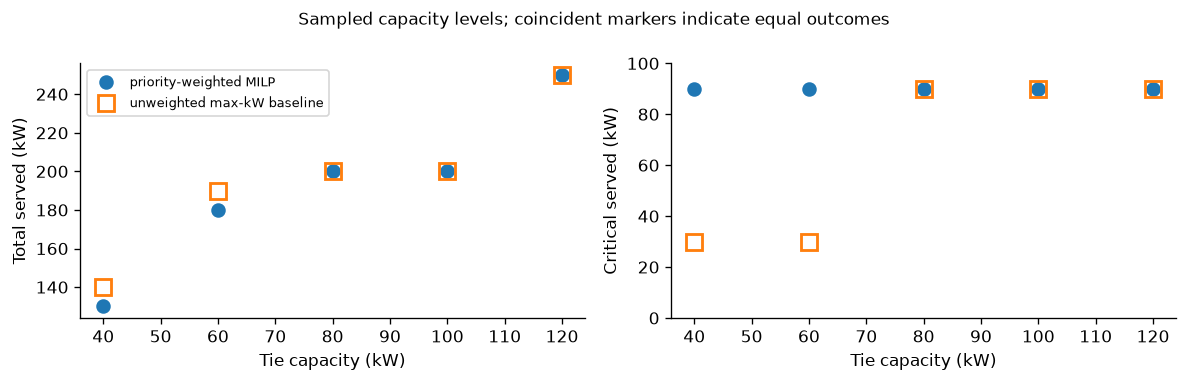
\includegraphics[width=.87\linewidth,height=3.4cm,keepaspectratio]{figures/classroom_restoration.png}\end{center}
\Idea{Two ratings, same pickup}{At 80 and 100 kW: weighted service is 200 kW total, including all 90 critical kW.}
\Question{Is the flat step evidence that capacity has no value?}
\Answer{No. It reflects indivisible load blocks and the available routes at these sampled ratings.}
\Source{Original computed figure: Classroom\_Labs L6 / classroom\_restoration.png. Same feasible constraints; weighted versus unweighted objectives.}
\Bridge{Where do the five agent stages add structure to this calculation?}
\note{Point first to the axes and the discrete sample markers. The plot compares policy choices at a set of tie capacities, not a continuously optimized physical design. At eighty and one hundred kilowatts, the weighted solution serves two hundred kilowatts in total and all ninety kilowatts of critical demand. A rating increase does not always admit another indivisible load block. The figure also lets participants see where objectives coincide, which is as important as the point where they differ. Do not interpret coincident markers as evidence that only one method ran. Both outcomes are plotted. Ask a participant to relate one marker back to a feasible path and the branch bottleneck from the earlier diagrams. Finish by distinguishing optimization quality from workflow quality: the next slide shows how the calculation becomes a traceable proposal, with assumptions and checks attached.}
\end{frame}

\begin{frame}[t]{The workflow surrounds the solver with evidence and decisions}
\label{f:R13}
\small
\renewcommand{\arraystretch}{1.12}
\begin{tabularx}{\linewidth}{>{\bfseries\raggedright\arraybackslash}p{2.35cm}>{\raggedright\arraybackslash}p{4.4cm}>{\raggedright\arraybackslash}X}
\toprule Stage & Specific method & Output that can be checked\\\midrule
Awareness & Topology and status checks & Fault 1--2; ratings; critical nodes 2, 5\\
Planning & Weighted restoration MILP & Pickup vector and selected edges\\
Simulation & Active-power transport & Per-edge demand and capacity margins\\
Verification & Independent enumeration & Feasible and objective agreement\\
LLM Optimizer & Allowed refinement request & Proposed next calculation, with rationale\\\bottomrule
\end{tabularx}
\uncover<2->{\Idea{Scope matters}{L6--L7 run fresh numerical and binding checks. L10 replays the full five-stage language trace from the separate archived feeder experiment.}}
\Source{Classroom\_Labs L6--L7, L10; proposal\_complete\_workflow.json. This table describes stage roles; L6 does not make five live LLM calls.}
\Bridge{What happens when the network rating changes after verification?}
\note{Read each row as a method producing a concrete output, rather than as five people having a conversation. Awareness binds the request to a topology and trusted ratings. Planning chooses pickups and edges. Simulation evaluates the transport consequences. Verification checks feasibility and, in this small case, agreement with an exhaustive optimum. The LLM optimizer may propose an allowed refinement or explain a tool result, but it does not override a failed capacity check. Be precise about what students are executing. L6 and L7 provide fresh numerical and evidence-binding experiments. L10 displays the full archived five-stage trace from a different feeder fixture. It would be misleading to imply that L6 itself makes all those language calls. The common framework is the contract among stages, while the physical models and numerical methods vary with the task.}
\end{frame}

\begin{frame}[fragile,t]{Hands-on: old evidence does not certify a changed rating}
\label{f:R14}
\Checkpoint{L7}{Four minutes: run the full cell, then explain the two Boolean results.}
\lstinputlisting[style=python,firstline=7,lastline=10]{snippets/L7.py}
\begin{center}
\begin{tikzpicture}[node distance=.8cm]
\node[box,text width=3cm] (a) {revision 1\\40 kW tie};
\node[box,text width=3.5cm,right=of a] (b) {candidate + evidence\\bound to revision 1};
\node[box,text width=3cm,right=of b,draw=red] (c) {revision 2\\20 kW tie};
\draw[arrow] (a)--(b);\draw[arrow,red] (b)--node[above,font=\small]{reuse?}(c);
\end{tikzpicture}
\end{center}
\Answer{Original binding: True. Changed request with old evidence: False. HOLD and re-solve.}
\Source{Exact excerpt: Classroom\_Labs L7 lines 7--10; lab.bind\_evidence and lab.bound\_to. Binding checks identity, not physical feasibility by itself.}
\Bridge{What additional evidence appears in the larger archived feeder case?}
\note{This exercise tests a workflow failure that can occur even when the original optimizer worked perfectly. The request changes from a forty-kilowatt tie rating at revision one to twenty kilowatts at revision two. The previous candidate and its evidence remain associated with the original request. The binding check should return true for that original request and false for the changed request. That failure means the old result is not valid evidence for the new contract; it does not independently prove that the old pickup is physically infeasible. A new constrained solve is required to decide that. Ask participants to name other changes that should invalidate evidence, such as topology, priorities, measurement provenance or the model version. The intended benefit is preventing stale recommendations from being presented as current checked actions, not improving the MILP objective.}
\end{frame}

\begin{frame}[t]{Archived feeder: an attractive pickup can fail a thermal check}
\label{f:R15}
\begin{columns}[T,onlytextwidth]
\column{.51\textwidth}
\begin{tikzpicture}[x=.032cm,y=1cm]
\fill[red!65] (0,0) rectangle (151.639,.65);
\draw[red,thick,dashed] (100,-.15)--(100,1);
\node[font=\scriptsize,above] at (100,1) {100\% limit};
\node[font=\small,below] at (75,-.25) {E01: 151.64\% loading};
\node[box,text width=4.8cm] at (75,-1.45) {Verification rejects the initial high-pickup proposal.};
\end{tikzpicture}
\column{.46\textwidth}
\Idea{Different fixture; explicit scope}{Archived MV feeder; synthetic short bypass; 100 A limit; ideal LV aggregation. No time-ordered switching certificate.}
\uncover<2->{\Idea{Refine, simulate, verify again}{A permitted shedding refinement produces a passing candidate: 1843.61 kW served, including 474.04 kW critical.}}
\end{columns}
\Source{ARCHIVED ACTUAL: proposal\_complete\_workflow.json, restoration / lindistflow3. Initial E01 loading 151.639\%; final verified SHED\_075.}
\Bridge{What did Llama actually say, and which statement required correction?}
\note{Make the fixture change explicit before presenting the numbers. We have left the six-node classroom graph and are inspecting an archived medium-voltage feeder workflow. It has a synthetic bypass catalog and an ideal low-voltage aggregation assumption. In the LinDistFlow3 run, the initial high-pickup candidate overloads the bypass to about one hundred fifty-two percent of its rating. That numerical result triggers rejection regardless of its language explanation. A permitted refinement sheds a specified fraction of ordered noncritical load objects, after which a candidate passes the modeled constraints. The final served and critical-service values belong only to this archive. They should not be combined with the six-node optimum table. The trace demonstrates rejection, refinement and rechecking. It does not establish a safe field switching sequence, protection coordination or a deployed operator decision.}
\end{frame}

\begin{frame}[t]{Llama can request a useful check and still rank results incorrectly}
\label{f:R16}
\small
\Idea{Actual Planning response: 0.874 s}{\textit{``Requesting both initial simulations as per the Planning Agent's role and the contract's operational limit.''}}
\uncover<2->{\Idea{Actual LLM ranking: numerical guard required}{Returned ranking: E02, E03.\par Returned scores: E02 $=-5509.14$; E03 $=-6109.97$.\par The task minimizes cost, so \textbf{E03 must precede E02}.}}
\Question{Should a majority of similar language responses overrule the score?}
\uncover<3->{\textcolor{teal}{No. Recompute the ordering from verified numerical evidence.}\par The accepted proposal is tied to a fresh final verification.}
\Source{Exact Planning quote and returned ranking: archived restoration / lindistflow3 trace, proposal\_complete\_workflow.json. Times are recorded model-call wall times.}
\Bridge{Does the matched fixed supervisor achieve a different final outcome?}
\note{Read the planning response exactly as recorded, without presenting it as hidden chain-of-thought. It is an observable rationale for requesting tools. The call took about eight hundred seventy-four milliseconds in the archived environment. The later language ranking provides a useful counterexample to treating fluency as numerical reliability. The returned sequence places E02 before E03 even though the objective is minimized and E03 has the more negative score. A deterministic ranking guard corrects that ordering using verified values. Multiple similar LLM votes would not make the incorrect comparison true. This is a concrete workflow benefit: language proposes and explains, while explicit numerical rules constrain acceptance. It is also a limitation of the language component. The final candidate receives fresh verification, so acceptance is attached to evidence rather than to a persuasive ranking statement alone.}
\end{frame}

\begin{frame}[t]{Matched supervision: equal service, different latency}
\label{f:R17}
\small
\begin{center}
\begin{tabular}{lrr}
\toprule Archived LinDistFlow3 restoration & Fixed supervisor & Llama supervisor\\\midrule
Total served (kW) & 1843.61 & 1843.61\\
Critical served (kW) & 474.04 & 474.04\\
Objective cost & $-6109.97$ & $-6109.97$\\
Total elapsed time (s) & 0.306 & 5.232\\\bottomrule
\end{tabular}
\end{center}
\uncover<2->{\Idea{A result worth teaching honestly}{This run shows no service improvement from Llama. Its visible contribution is a tool-selection rationale and trace; it adds latency and needs numerical guards.}}
\Question{What would demonstrate an additional agentic benefit?}
\Answer{Matched tests of changed requests, tool failures and stale evidence, with success rate and human effort measured.}
\Source{ARCHIVED ACTUAL: fixed versus agentic, restoration / lindistflow3, proposal\_complete\_workflow.json. Single recorded case; four Llama calls.}
\Bridge{What should the operator receive before any restoration action?}
\note{This is the controlled comparison within the archived restoration setup. Both supervisors use the same final physical task, candidate tools, constraints and cost definition. They reach the same final service and objective. The language-driven supervisor takes substantially longer in this single recorded run. Avoid describing the ratio as a general benchmark; model loading, hardware, caching and task difficulty can change latency. The trace is useful for seeing what was requested, why the high-pickup candidate failed, and how a later candidate was checked. That usefulness must be measured separately from electrical performance. Suggest future matched evaluations involving changed ratings, failed tools and stale evidence, with explicit acceptance rules and operator workload measures. Do not imply these tests already demonstrate superiority. The honest conclusion is that this case exposes workflow behavior and limitations while preserving the conventional numerical result.}
\end{frame}

\begin{frame}[t]{Handoff: show the action, the evidence and the remaining decision}
\label{f:R18}
\begin{center}
\begin{tikzpicture}[node distance=.55cm]
\node[box,text width=3.45cm] (a) {Proposed pickup and paths\\objective and priorities};
\node[box,text width=3.45cm,right=of a] (b) {Current checks\\ratings, revision, model scope};
\node[box,text width=3.45cm,right=of b] (c) {Operator decision\\acknowledge, revise, reject};
\draw[arrow] (a)--(b);\draw[arrow] (b)--(c);
\end{tikzpicture}
\end{center}
\Idea{A complete recommendation is conditional}{State which measurements and equipment statuses were trusted. A passing calculation is tied to that information and that model.}
\Question{What if the network model is correct but the measurements are deceptive?}
\Answer{The planner may optimize the wrong state. The next case tests consistency, observability and trusted replacement evidence.}
\Source{Restoration lessons: Classroom\_Labs L6--L7 and archived L10 trace. Operator acknowledgment is a tutorial workflow, not a field execution system.}
\Bridge{Can internally consistent measurements still describe the wrong state?}
\note{Close restoration with the operator's view. A recommendation should identify what demand is restored, what topology it assumes, the service priorities, the modeled limits and the evidence revision. It should also state what was not certified, especially switching sequence and protection behavior in these exercises. Acknowledgment is not merely clicking through a green badge; it is a decision made with those conditions visible. Participants have now seen two complementary benefits: an optimization objective that protects designated demand, and a workflow that prevents stale or failed evidence from being treated as valid. Neither requires claiming that Llama improves the optimum. Use the final question as the transition to cyber response. Even a correct network model and a competent optimizer can recommend the wrong action when measurements describe the wrong state. The next lesson separates consistency from trust.}
\end{frame}
